\section*{Определение требований}

В рамках построения эллиптических кривых с комплексным умножением существует общий подход, предложенный А.Ю. Нестеренко. В данной работе рассматривается специфический случай, когда коэффициенты \( a \) и \( b \), эндоморфизм, а также число классов уже известны. Основная задача заключается в подборе такого простого числа \( p \), которое удовлетворяет следующим условиям:

\begin{enumerate}
    \item Условие для существования эндоморфизма в виде комплексного умножения: Символ Лежандра \((d|p)\) должен быть равен 1.
    \item Условие для существования отображения в форму Хадано: Символ Лежандра \((\gamma|p)\) должен быть равен 1.
    \item Условие для существования отображения в форму Скрученного Эдвардса: Из уравнения Корначи \(x^2 + dy^2 = 4p\) находим \(x\). Затем, определяем \(m_{\Delta} = p + 1 + x\), и устанавливаем, что \(m_{\Delta} = mq\), где \(m\) должен быть равен \(4\) для существования перевода в форму Скрученного Эдвардса, при этом \(q\) являться простым числом.
\end{enumerate}

Рассмотрим данные условия на примере \( d = -3, \gamma = 2 \).

Символ Лежандра \((-3|p)\) определяется для нечетного простого \(p\) и целого \(a\), и он равен 1, если \(a\) является квадратичным вычетом по модулю \(p\). Для \(d = -3\), мы хотим узнать, при каких условиях на \(p\), \(-3\) является квадратичным вычетом.

Квадратичный закон взаимности гласит, что для двух нечетных простых чисел \(p\) и \(q\):
\[
(p|q) =
\begin{cases}
(q|p), & \text{если одно из чисел } p \text{ или } q \equiv 1 \mod 4,\\
-(q|p), & \text{в противном случае}.
\end{cases}
\]

Свойства символа Лежандра:
\begin{itemize}
\item \( (-1|p) = 1 \), если \( p \equiv 1 \mod 4 \); \( -1 \), если \( p \equiv 3 \mod 4 \).
\item \( (3|p) = 1 \), если \( p \equiv 1 \mod 3 \); \( -1 \), если \( p \equiv -1 \mod 3 \).
\end{itemize}

Таким образом, \((-3|p) = (-1|p) \times (3|p)\). Чтобы \((-3|p) = 1\), оба символа Лежандра должны быть либо оба равны 1, либо оба равны -1. Это достигается, когда \( p \) удовлетворяет одному из следующих условий:
\begin{itemize}
    \item \( p \equiv 1 \mod 12 \), так как \( p \equiv 1 \mod 4 \) и \( p \equiv 1 \mod 3 \), что удовлетворяет обоим условиям.
    \item \( p \equiv 7 \mod 12 \), так как \( p \equiv 3 \mod 4 \) и \( p \equiv -1 \mod 3 \), что также удовлетворяет обоим условиям.
\end{itemize}

Аналогично для \(\left(\frac{2}{p}\right)\). Он равен 1, если \(p \equiv \pm 1 \mod 8\), и равен -1, если \(p \equiv \pm 3 \mod 8\).

Следовательно, для того чтобы \((-3|p) = 1\) и \((2|p) = 1\), простое число \(p\) должно удовлетворять одному из условий: \(p \equiv 1 \mod 24\) или \(p \equiv 7 \mod 24\).

Следующим шагом в построении эллиптической кривой является решение уравнения \( x^2 - d*y^2 = 4p \). Значение \( x \), полученное из этого уравнения, используется для определения порядка кривой.

\textbf{Алгоритм Корначи для решения уравнения.} Алгоритм Корначи – это эффективный метод для решения квадратных уравнений вида \( x^2 - Dy^2 = N \), где \( D \) и \( N \) – целые числа.~\cite{cohen-cornach}

\textbf{Применение найденного значения \( x \).} Значение \( x \), полученное из уравнения, используется для вычисления порядка эллиптической кривой через формулу \( m_{\Delta} = p + 1 + x =  m * q\) ~\cite{nesterenko-disser}. Это позволяет определить точное количество точек \( q \) на соответствующей эллиптической кривой.

\textbf{Значение \( m = 4 \) и выбор простого числа \( q \).} Выбор \( m = 4 \) в формуле \( m_{\Delta} = 4q \) обусловлен необходимостью обеспечения возможности перехода к форме Эдвардса эллиптической кривой. Выбор простого числа \( q \) критичен для обеспечения криптографической стойкости кривой.

\section*{Полученные результаты}
В результате была построена эллиптическая кривая по указанным требованиям в размерности 256 бит. 

\begin{table}[h]
  \centering
  \begin{tabular}{cl}
      \hline
      \textbf{Ключ} & \textbf{Значение} \\
      \hline
      point.x & 1 \\
      point.y & 1370184815209153778412612456839413869416711536549829925085495630500881379458 \\
      point.z & 1 \\
      a & $2^{253} + 83372$ \\
      b & $2^{253} + 83373$ \\
      p & $2^{255} + 333503$ \\
      q & $2^{253} + 119232052797507057057440919387189651419$ \\
      \hline
  \end{tabular}
  \caption{Параметры построенной эллиптической кривой 256 бит}
\end{table}

Эллиптическая кривая 256 бит.



Сравнение результатов количества действий в разных кривых на разных операциях:


\begin{table}[h]
  \centering
  \begin{tabular}{|c|c|c|}
    \hline
    \textbf{Операция} & \textbf{Сложения} & \textbf{Умножения} \\
    \hline
    Эндоморфизм в форме Хадано & 5 & 13 \\
    \hline
    Вейерштрасс (сложение точек) & 7 & 14 \\
    \hline
    Вейерштрасс (удвоение точки) & 10 & 13 \\
    \hline
    Монтгомери (сложение) & 6 & 6 \\
    \hline
    Монтгомери (удвоение) & 4 & 5 \\
    \hline
    Хадано (сложение) & 7 & 18 \\
    \hline
    Хадано (удвоение) & 10 & 17 \\
    \hline
    Скрученный Эдвардс (сложение) & 6 & 13 \\
    \hline
    Скрученный Эдвардс (удвоение) & 6 & 9 \\
  \hline
  \end{tabular}
  \caption{Количество действий в операциях в разных формах эллиптических кривых}
\end{table}

Для проведения эксперимента в рамках дипломной работы был использован следующий алгоритм:

\begin{enumerate}
    \item Установить $i$ в диапазоне от 2 до 74 (включительно).
    \item Вычислить $j$ как округленное значение логарифма по основанию 2 от $10^i$, умноженное на 2.
    \item Инициализировать пустой список $numbers$ для хранения чисел.
    \item Для каждого значения $j$:
        \begin{enumerate}
            \item Сгенерировать случайное целое число $x$ в диапазоне от $10^i$ до $10^{(i+1) - 1}$.
            \item Добавить $x$ в список $numbers$.
        \end{enumerate}
\end{enumerate}

Этот алгоритм использовался для подготовки данных для дальнейших сравнений. Он включал в себя генерацию случайных целых чисел в заданных диапазонах для различных степеней 10. Полученные числа использовались в дипломной работе для проведения экспериментов и анализа результатов.


\pagebreak
Сравнение результатов подсчета количества умножений в каждой из форм 
\begin{figure}[h]
  \centering
  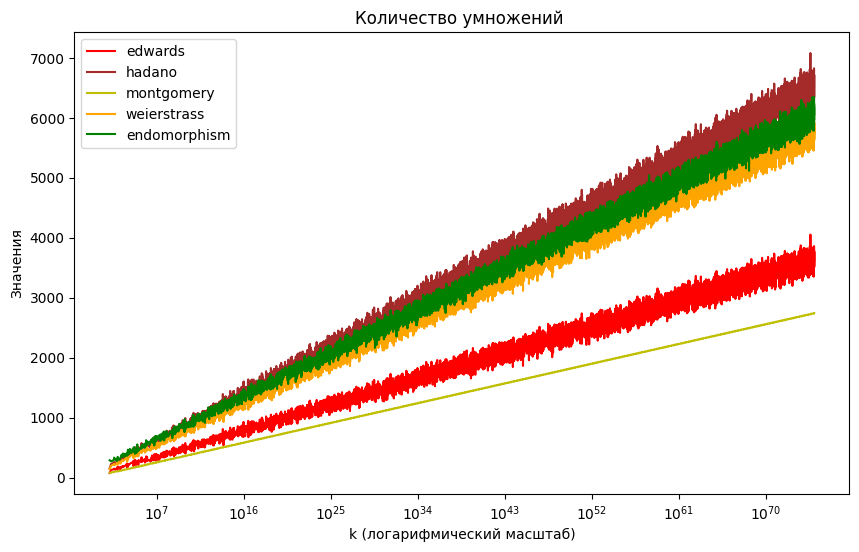
\includegraphics[width=\linewidth]{./multiplication.png}
  \caption{Связь количества умножений от формы кривой и выбранной кратной точки}
  % \label{fig:my_label}
  \end{figure}

Экспериментальные исследования показали, что среди выбранных форм, эллиптические кривые в форме Монтгомери и в форме Эдвардса имеют наименьшее количество умножений. Эллиптическая кривая в форме Хадано с изучаемым эндоморфизмом имеет незначительно больше умножений чем форма Вейештрасса.

В среднем, кривая в форме Монтгомери эффективнее кривой в форме Скрученного Эдвардса на 30\%, эффективнее формы Вейештрасса на 110\%, эффективнее формы Хадано с эндоморфизмом на 120\% и эффективнее формы Хадано без эндоморфизма на 135\%.

\pagebreak

Сравнение результатов подсчета количества сложений в каждой из форм 
\begin{figure}[h]
  \centering
  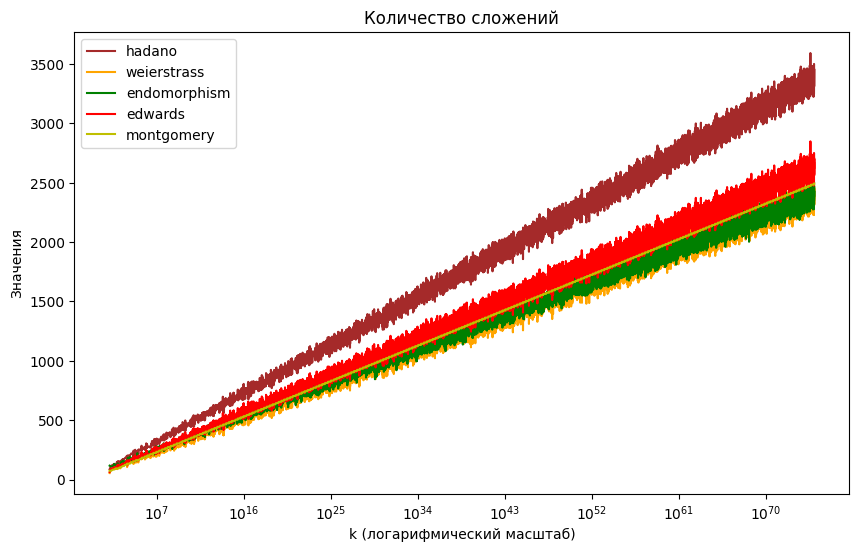
\includegraphics[width=\linewidth]{./additions.png}
  \caption{Связь количества сложений от формы кривой и выбранной кратной точки}
  % \label{fig:my_label}
  \end{figure}

Экспериментальные исследования показали, что среди выбранных форм, эллиптические кривые в форме Вейештрасса и в форме Хадано с эндоморфизмом имеют наименьшее количество сложений. Следом идут форма Монтгомери и форма Скрученного Эдвардса.

В среднем, кривая в форме Вейерштрасса эффективнее кривой в форме Скрученного Эдвардса на 10\%, эффективнее формы Хадано на 40\%, эффективнее формы Монтгомери на 5\% и эффективнее формы Хадано с эндоморфимом на 1\%.
\pagebreak
Для суммирования количества умножений и сложений было предложено сопоставить 1 умножение как 1.5 сложения для простоты. 
\begin{figure}[h]
  \centering
  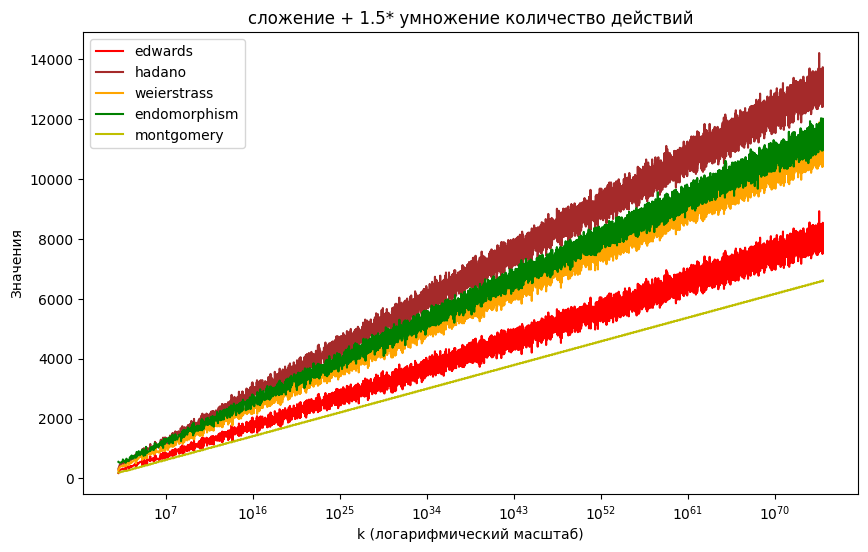
\includegraphics[width=\linewidth]{./add_and_mul.png}
  \caption{Связь количества умножений и сложений от формы кривой и выбранной кратной точки}
  % \label{fig:my_label}
  \end{figure}

Экспериментальные исследования показали, что среди выбранных форм, эллиптические кривые в форме Монтгомери и Эдвардса имеют суммарно наименьшее количество действий. Эллиптическая кривая в форме Вейештрасса и в форме Хадано с эндоморфизмом идут дальше и наименее эффективной является форма Хадано.


\pagebreak

Сравнение результатов подсчета времени в каждой из форм (усредненное для логарифма по основанию 10)
\begin{figure}[h]
  \centering
  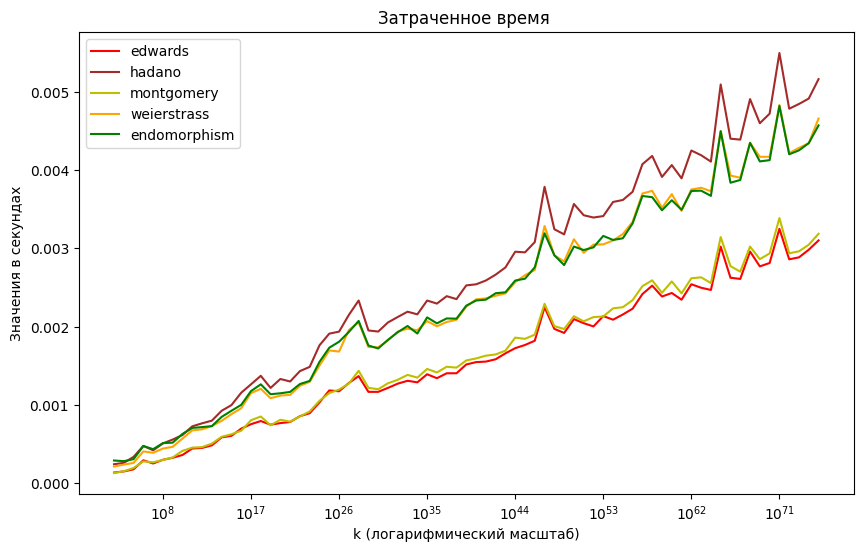
\includegraphics[width=\linewidth]{./time.png}
  \caption{Время в секундах, потраченное на возведение в кратную точку}
  % \label{fig:my_label}
  \end{figure}


В результате наиболее эффективными формами эллиптических кривых относительно времени выполнения являются форма Монтгомери и форма Скрученного Эдвардса. 

В среднем, кривая в форме Скрученного Эдвардса по времени эффективнее кривой в форме Хадано на 65\%, эффективнее формы Монтгомери на 2\%, эффективнее формы Хадано с эндоморфизмом на 50\% и эффективнее формы Вейерштрасса на 47\%.
